\documentclass[aspectratio=169, professionalfonts]{beamer}

\usetheme{Szeged}
\usecolortheme{dolphin}

\usepackage{amsmath, amssymb, bm}
\usepackage{tikz}
\usetikzlibrary{positioning, arrows.meta, decorations.pathreplacing, calc}
\usepackage{pgfplots}
\pgfplotsset{compat=1.18}

\def\R{\mathbb{R}}
\def\E{\mathbb{E}}

\definecolor{mantis}{RGB}{0, 105, 62}

\setbeamercolor{frametitle}{fg=white, bg=mantis}
\setbeamercolor{title}{fg=white, bg=mantis}
\setbeamercolor{structure}{fg=mantis}
\setbeamercolor{block title}{bg=mantis, fg=white}
\setbeamercolor{block body}{bg=mantis!10}

\title{Neural Networks \& Backpropagation}
\subtitle{From the Perceptron to Deep Learning}
\author{Lebnet Tech Fellows Program}
\date{}

\begin{document}

% ------------------------------------------------------------------
\begin{frame}
\titlepage
\end{frame}

% ------------------------------------------------------------------
\begin{frame}{Roadmap}
\tableofcontents
\end{frame}

% ==================================================================
\section{The Perceptron}
% ==================================================================

% ------------------------------------------------------------------
\begin{frame}{A Neuron-Inspired Classifier}

Given labelled data $(x, l(x))$ with $x \in \R^n$, $l(x) \in \{+1,-1\}$:

$$l(x) = \text{sign}(\langle w^*, x \rangle)$$

$w^*$ is the normal vector to a separating hyperplane.

\bigskip

\begin{block}{Perceptron Algorithm}
\begin{enumerate}
  \item Initialise $w = 0$
  \item For each input $x$:
    predict $\text{sign}(\langle w, x \rangle)$;
    on a mistake, update $w \leftarrow w + l(x)\,x$
\end{enumerate}
\end{block}

\bigskip

Each update \textbf{tilts the hyperplane} toward the misclassified point.

\end{frame}

% ------------------------------------------------------------------
\begin{frame}{Visualising the Margin}

\begin{center}
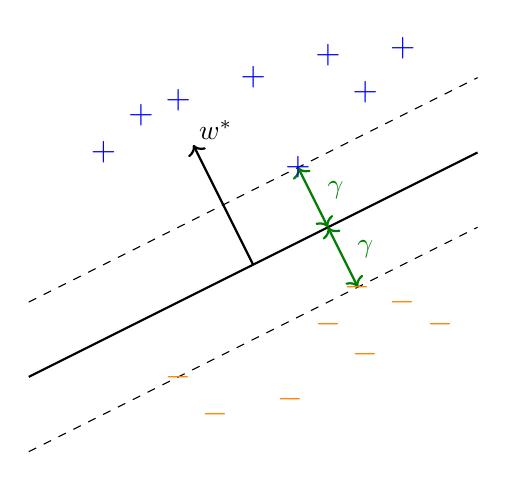
\begin{tikzpicture}[scale=0.95]
    \draw[thick, black] (-3,-1.5) -- (3,1.5);
    \draw[dashed, black] (-3,-0.5) -- (3,2.5);
    \draw[dashed, black] (-3,-2.5) -- (3,0.5);
    \draw[->, thick, black] (0,0) -- (-0.8,1.6);
    \node[black] at (-0.5,1.8) {$w^*$};
    \draw[<->, thick, green!50!black] (1,0.5) -- (0.6,1.3);
    \node[green!50!black] at (1.1,1.0) {$\gamma$};
    \draw[<->, thick, green!50!black] (1,0.5) -- (1.4,-0.3);
    \node[green!50!black] at (1.5,0.2) {$\gamma$};
    \node[blue, font=\bfseries\large] at (-2,1.5) {$+$};
    \node[blue, font=\bfseries\large] at (-1,2.2) {$+$};
    \node[blue, font=\bfseries\large] at (0,2.5) {$+$};
    \node[blue, font=\bfseries\large] at (1,2.8) {$+$};
    \node[blue, font=\bfseries\large] at (0.6,1.3) {$+$};
    \node[blue, font=\bfseries\large] at (1.5,2.3) {$+$};
    \node[blue, font=\bfseries\large] at (-1.5,2.0) {$+$};
    \node[blue, font=\bfseries\large] at (2,2.9) {$+$};
    \node[orange, font=\bfseries\large] at (2,-0.5) {$-$};
    \node[orange, font=\bfseries\large] at (1,-0.8) {$-$};
    \node[orange, font=\bfseries\large] at (1.4,-0.3) {$-$};
    \node[orange, font=\bfseries\large] at (-1,-1.5) {$-$};
    \node[orange, font=\bfseries\large] at (1.5,-1.2) {$-$};
    \node[orange, font=\bfseries\large] at (2.5,-0.8) {$-$};
    \node[orange, font=\bfseries\large] at (0.5,-1.8) {$-$};
    \node[orange, font=\bfseries\large] at (-0.5,-2.0) {$-$};
\end{tikzpicture}
\end{center}

The margin $\gamma$ is the minimum distance from any point to the
decision boundary. Larger margin $\Rightarrow$ fewer mistakes.

\end{frame}

% ------------------------------------------------------------------
\begin{frame}{Convergence Guarantee}

\begin{definition}[Margin]
$\gamma := \min_{x \in D} |\langle w^*, x \rangle|$
\quad (assuming $\|w^*\|=1$, $\|x\|\le 1$)
\end{definition}

\bigskip

\begin{alertblock}{Perceptron Convergence Theorem}
The number of mistakes is at most $\dfrac{1}{\gamma^2}$.
\end{alertblock}

\bigskip

\textbf{Proof idea:} track $\cos(w, w^*)$.
Each mistake grows the numerator by $\ge\gamma$
but the denominator by $\le\sqrt{T}$.
Cauchy-Schwarz forces $T \le 1/\gamma^2$.

\end{frame}

% ==================================================================
\section{The Limits of Linearity}
% ==================================================================

% ------------------------------------------------------------------
\begin{frame}{Linear Models Cannot Be Stacked}

\begin{alertblock}{Key Fact}
A composition of linear (affine) functions is still linear:
$$(g \circ f)(x) = (CA)x + (Cb + d)$$
\end{alertblock}

\bigskip

A 100-layer linear network $=$ a single-layer network.

\bigskip

To learn nonlinear decision boundaries we need
\textbf{activation functions} applied element-wise:

$$h^{(l)} = \sigma\!\bigl(W^{(l)} h^{(l-1)} + b^{(l)}\bigr)$$

\end{frame}

% ------------------------------------------------------------------
\begin{frame}{Common Activation Functions}

\begin{columns}[c]
\column{0.4\textwidth}
\begin{center}
\small
\begin{tabular}{ll}
\textbf{Name} & \textbf{Definition} \\[4pt]
Sigmoid & $\frac{1}{1+e^{-z}}$ \\[6pt]
Tanh & $\frac{e^z - e^{-z}}{e^z + e^{-z}}$ \\[6pt]
ReLU & $\max(0, z)$ \\[6pt]
Leaky ReLU & $\max(\alpha z, z)$
\end{tabular}
\end{center}

\column{0.6\textwidth}
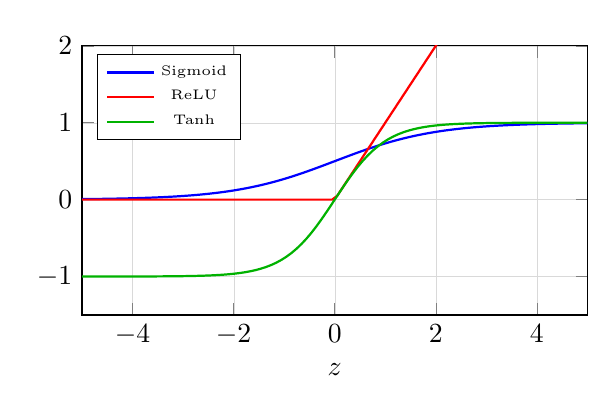
\begin{tikzpicture}
\begin{axis}[
    width=8cm, height=5cm,
    xlabel={$z$},
    xmin=-5, xmax=5, ymin=-1.5, ymax=2,
    legend style={font=\tiny, at={(0.03,0.97)}, anchor=north west},
    grid=both,
    grid style={line width=.1pt, draw=gray!30},
]
\addplot[domain=-5:5, samples=100, color=blue, thick]
  {1/(1+exp(-x))};
\addplot[domain=-5:5, samples=100, color=red, thick]
  {max(0,x)};
\addplot[domain=-5:5, samples=100, color=green!70!black, thick]
  {tanh(x)};
\legend{Sigmoid, ReLU, Tanh}
\end{axis}
\end{tikzpicture}
\end{columns}

\end{frame}

% ==================================================================
\section{Universal Approximation}
% ==================================================================

% ------------------------------------------------------------------
\begin{frame}{Neural Nets Can Approximate Anything}

\begin{block}{Universal Approximation Theorem}
For any continuous $f:[0,1]^d\to\R$ and any $\varepsilon>0$,
there exists a single-hidden-layer network
$$g(x) = \sum_{j=1}^{N} c_j\,\sigma(\langle w_j, x\rangle + b_j)$$
such that $\sup_x |f(x) - g(x)| < \varepsilon$.
\end{block}

\bigskip

Holds for any continuous, non-polynomial activation
(sigmoid, tanh, ReLU, \ldots).

\end{frame}

% ------------------------------------------------------------------
\begin{frame}{Intuition: ReLU Bump Functions}

Two ReLUs make a bump; scaled bumps approximate any curve.

\begin{columns}[c]
\column{0.5\textwidth}
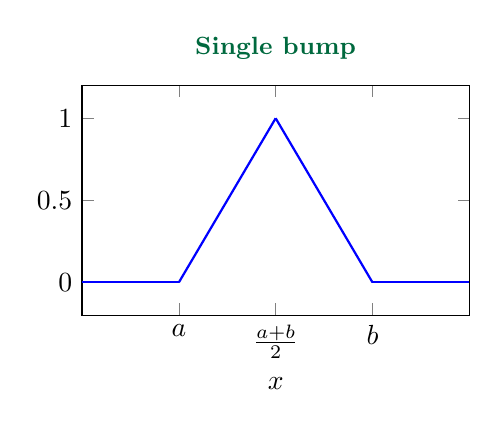
\begin{tikzpicture}
\begin{axis}[
    width=6.5cm, height=4.5cm,
    xlabel={$x$},
    xmin=-0.5, xmax=3.5, ymin=-0.2, ymax=1.2,
    xtick={0.5,1.5,2.5},
    xticklabels={$a$,$\frac{a+b}{2}$,$b$},
    title style={font=\small\bfseries\color{mantis}},
    title={Single bump},
]
\addplot[domain=-0.5:0.5, samples=10, color=blue, thick] {0};
\addplot[domain=0.5:1.5, samples=10, color=blue, thick] {x-0.5};
\addplot[domain=1.5:2.5, samples=10, color=blue, thick] {2.5-x};
\addplot[domain=2.5:3.5, samples=10, color=blue, thick] {0};
\end{axis}
\end{tikzpicture}

\column{0.5\textwidth}

\begin{itemize}
  \item Partition $[0,1]$ into $n$ intervals
  \item Place a scaled bump on each interval
  \item Piecewise linear $\to$ arbitrary precision
        by uniform continuity
\end{itemize}
\end{columns}

\bigskip

A network with $n$ hidden ReLU units can represent any
piecewise linear function with $n$ pieces.

\end{frame}

% ------------------------------------------------------------------
\begin{frame}{Example: Approximating a Function with ReLU Bumps}

\begin{center}
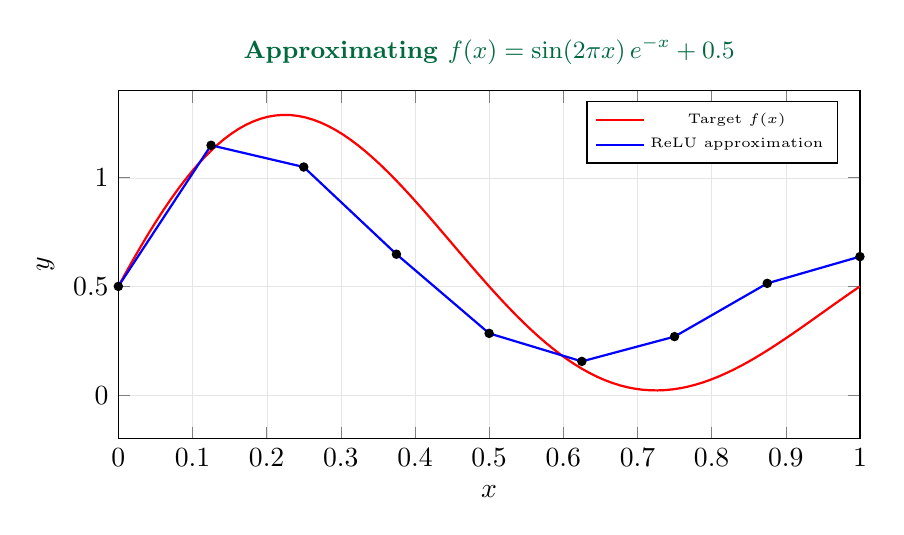
\begin{tikzpicture}
\begin{axis}[
    width=11cm, height=6cm,
    xlabel={$x$}, ylabel={$y$},
    xmin=0, xmax=1, ymin=-0.2, ymax=1.4,
    title={\textbf{Approximating $f(x) = \sin(2\pi x)\,e^{-x}+0.5$}},
    title style={font=\small\bfseries\color{mantis}},
    grid=both,
    grid style={line width=.1pt, draw=gray!20},
    legend style={font=\tiny, at={(0.97,0.97)}, anchor=north east},
]
\addplot[domain=0:1, samples=100, color=red, thick]
  {sin(deg(2*pi*x))*exp(-x)+0.5};
\addlegendentry{Target $f(x)$}
\addplot[domain=0:0.125, samples=10, color=blue, thick]
  {0.5+(0.5+0.649-0.5)/(0.125)*(x-0)};
\addplot[domain=0.125:0.25, samples=10, color=blue, thick]
  {0.5+0.649+(0.5+0.549-0.5-0.649)/(0.125)*(x-0.125)};
\addplot[domain=0.25:0.375, samples=10, color=blue, thick]
  {0.5+0.549+(0.5+0.148-0.5-0.549)/(0.125)*(x-0.25)};
\addplot[domain=0.375:0.5, samples=10, color=blue, thick]
  {0.5+0.148+(0.5-0.216-0.5-0.148)/(0.125)*(x-0.375)};
\addplot[domain=0.5:0.625, samples=10, color=blue, thick]
  {0.5-0.216+(0.5-0.345-0.5+0.216)/(0.125)*(x-0.5)};
\addplot[domain=0.625:0.75, samples=10, color=blue, thick]
  {0.5-0.345+(0.5-0.231-0.5+0.345)/(0.125)*(x-0.625)};
\addplot[domain=0.75:0.875, samples=10, color=blue, thick]
  {0.5-0.231+(0.5+0.014-0.5+0.231)/(0.125)*(x-0.75)};
\addplot[domain=0.875:1, samples=10, color=blue, thick]
  {0.5+0.014+(0.5+0.137-0.5-0.014)/(0.125)*(x-0.875)};
\addlegendentry{ReLU approximation}
\addplot[only marks, mark=*, mark size=1.5pt, color=black]
  coordinates {(0,0.5)(0.125,1.149)(0.25,1.049)(0.375,0.648)
               (0.5,0.284)(0.625,0.155)(0.75,0.269)(0.875,0.514)(1,0.637)};
\end{axis}
\end{tikzpicture}
\end{center}

More bumps (= more hidden units) $\Rightarrow$ tighter fit.

\end{frame}

% ==================================================================
\section{Training: Loss and Optimisation}
% ==================================================================

% ------------------------------------------------------------------
\begin{frame}{The Training Objective}

Network $f_\theta:\R^d\to\R^k$ with weights $\theta$,
training data $\{(x_i, y_i)\}_{i=1}^n$.

$$\mathcal{L}(\theta)
  = \frac{1}{n}\sum_{i=1}^{n}\ell\!\bigl(f_\theta(x_i),\, y_i\bigr)$$

\bigskip

\begin{center}
\small
\begin{tabular}{lll}
\textbf{Task} & \textbf{Loss} & \textbf{Formula} \\[2pt]
Regression & MSE &
  $\frac{1}{2}\|\hat{y}-y\|^2$ \\[4pt]
Binary classif.\ & Cross-entropy &
  $-y\log\hat{y}-(1-y)\log(1-\hat{y})$ \\[4pt]
Multi-class & Softmax CE &
  $-\log(\text{softmax}(\hat{y})_y)$
\end{tabular}
\end{center}

\end{frame}

% ------------------------------------------------------------------
\begin{frame}{SGD: Scalable Optimisation}

\textbf{Full gradient descent:}
$\;\theta_{t+1} = \theta_t - \eta\,\nabla\mathcal{L}(\theta_t)$
\quad (cost $O(n)$ per step)

\bigskip

\textbf{Stochastic gradient descent:} sample one (or a mini-batch of)
data point(s):
$$\theta_{t+1} = \theta_t
  - \eta_t\,\nabla\ell\!\bigl(f_{\theta_t}(x_i),\, y_i\bigr)$$

\begin{itemize}
  \item \textbf{Unbiased:}
    $\E_i[\nabla\ell_i] = \nabla\mathcal{L}(\theta)$
  \item Cost $O(1)$ per step (vs.\ $O(n)$)
  \item Converges with decaying learning rate
\end{itemize}

\end{frame}

% ==================================================================
\section{Backpropagation}
% ==================================================================

% ------------------------------------------------------------------
\begin{frame}{The Gradient Problem}

A neural network is a \textbf{computational graph} (DAG).

\bigskip

\textbf{Goal:} compute $\dfrac{\partial\mathcal{L}}{\partial w}$
for every weight $w$.

\bigskip

By the chain rule at node $v$ with downstream children $w_1,\dots,w_m$:

$$\frac{\partial f}{\partial v}
  = \sum_{j=1}^{m}
    \frac{\partial f}{\partial w_j}\cdot
    \frac{\partial w_j}{\partial v}$$

\bigskip

\textbf{Forward mode:} propagate $\frac{\partial v}{\partial\theta}$
forward for \emph{each} weight. Cost: $O(WE)$.

\textbf{Problem:} terms like $\frac{\partial f}{\partial v}$ are
recomputed from scratch for every weight.

\end{frame}

% ------------------------------------------------------------------
\begin{frame}{Backward Mode: Share the Work}

\textbf{Key insight:} compute $\frac{\partial\mathcal{L}}{\partial v}$
for \emph{all} nodes in a single backward sweep.

\bigskip

\begin{block}{Backpropagation}
\textbf{Forward pass:} compute and store all activations $v^{(l)}$.

\textbf{Backward pass} (from output to input):
\begin{enumerate}
  \item $\delta^{(L)} = \frac{\partial\mathcal{L}}{\partial v^{(L)}}$
  \item For $l = L{-}1$ down to $1$:
  \begin{itemize}
    \item $\delta^{(l)}
      = (W^{(l+1)})^\top\delta^{(l+1)} \odot \sigma'(u^{(l)})$
    \item $\frac{\partial\mathcal{L}}{\partial W^{(l)}}
      = \delta^{(l)}(v^{(l-1)})^\top$
  \end{itemize}
\end{enumerate}
\end{block}

\end{frame}

% ------------------------------------------------------------------
\begin{frame}{Why Backprop Wins}

Each edge is visited \textbf{once} forward, \textbf{once} backward.

\bigskip

\begin{center}
\begin{tabular}{ll}
\textbf{Method} & \textbf{Cost} \\[2pt]
Numerical (finite diff.) & $O(WE)$ \\
Forward-mode autodiff & $O(WE)$ \\
\textbf{Backpropagation} & $\bm{O(E)}$
\end{tabular}
\end{center}

\bigskip

$W$ = number of weights, $E$ = number of edges.

Backprop is what makes training large networks feasible.

\end{frame}

% ==================================================================
\section{Going Deep: Challenges}
% ==================================================================

% ------------------------------------------------------------------
\begin{frame}{Vanishing Gradients}

With $L$ sigmoid layers, the gradient at layer $l$ involves:

$$\frac{\partial\mathcal{L}}{\partial W^{(l)}}
  \propto \prod_{k=l}^{L}\sigma'(u^{(k)})\cdot W^{(k)}$$

\bigskip

Since $\sigma'(z) = \sigma(z)(1-\sigma(z)) \le \frac{1}{4}$
for all $z$:

$$\left\|\frac{\partial\mathcal{L}}{\partial W^{(1)}}\right\|
  = O\!\left(\frac{1}{4^{L-1}}\right)$$

\bigskip

Gradients \textbf{shrink exponentially} with depth.
Early layers barely learn.

\end{frame}

% ------------------------------------------------------------------
\begin{frame}{Exploding Gradients}

If $\|W^{(k)}\| > 4$, the product grows exponentially instead:

$$\left\|\frac{\partial\mathcal{L}}{\partial W^{(1)}}\right\|
  = O(\lambda^{L-1}), \quad \lambda > 1$$

\bigskip

Weights oscillate wildly; training diverges.

\bigskip

\begin{alertblock}{The core tension}
Sigmoid derivatives are $\le 1/4$.
Multiply enough of them $\Rightarrow$ vanish.
Scale weights up to compensate $\Rightarrow$ explode.
\end{alertblock}

\end{frame}

% ------------------------------------------------------------------
\begin{frame}{Modern Solutions}

\begin{enumerate}
  \item \textbf{ReLU activation:}
    $\sigma'(z) \in \{0,1\}$, no shrinking in the active region.

  \bigskip

  \item \textbf{Careful initialisation:}
    \begin{itemize}
      \item Xavier (Glorot):
        $\text{Var}(w) = \frac{2}{n_{\text{in}}+n_{\text{out}}}$
        \quad(tanh/sigmoid)
      \item He:
        $\text{Var}(w) = \frac{2}{n_{\text{in}}}$
        \quad(ReLU)
    \end{itemize}

  \bigskip

  \item \textbf{Batch normalisation:}
    normalise activations per mini-batch to
    $\hat z = \frac{z-\mu_B}{\sqrt{\sigma_B^2+\epsilon}}$.

  \bigskip

  \item \textbf{Residual connections (ResNets):}
    $h^{(l+1)} = h^{(l)} + F(h^{(l)})$.
    Gradients flow through the identity path.
\end{enumerate}

\end{frame}

% ==================================================================
\section{The Big Picture}
% ==================================================================

% ------------------------------------------------------------------
\begin{frame}{The Progression of Ideas}

\begin{center}
\small
\begin{tabular}{lll}
\textbf{Model} & \textbf{Key Insight} & \textbf{Limitation} \\[2pt]
Perceptron & Linear separation &
  Only linearly separable data \\[4pt]
SVM & Max margin + kernels &
  Fixed feature space \\[4pt]
Neural Net & Nonlinear activations $\to$ UAT &
  Training is non-convex \\[4pt]
Deep Nets & Depth gives expressiveness &
  Vanishing/exploding gradients
\end{tabular}
\end{center}

\bigskip

\begin{block}{Key takeaways}
\begin{enumerate}
  \item Nonlinearity is \textbf{essential}: without it, depth is useless.
  \item One hidden layer \textbf{suffices} in theory (UAT),
        but depth helps in practice.
  \item Backprop computes all gradients in $O(E)$,
        making large-scale training possible.
  \item ReLU, good init, and residual connections
        tame the gradient flow.
\end{enumerate}
\end{block}

\end{frame}

% ------------------------------------------------------------------
{
\setbeamercolor{background canvas}{bg=mantis}
\setbeamercolor{normal text}{fg=white}
\usebeamercolor[fg]{normal text}
\begin{frame}[c]
\centering
\Huge\textbf{Questions?}
\end{frame}
}

\end{document}
